\newpage
%%%%%%%%%%%%%%%%%%%%%%%%%%%%
\section{Manejo del proyecto}
%%%%%%%%%%%%%%%%%%%%%%%%%%%%%

\subsection{Divisi\' on de los roles}
%%%%%%%%%%%%%%%%%%%%%%%%%%%%%%
Con respecto a la metodolog\' ia empleada en el presente laboratorio, se realiz\' o una divis\' on de tareas o roles que cada uno de los integrantes va a tomar, tal y como se puede observar en la siguiente lista:\\

\begin{itemize}
\item \textbf{Natalia Araya Campos}: \textit{Dise\~nadora}. Esta persona participar\' a activamente en todas las tareas que se requieran, sin embargo, tendr\'a un inter\'es enfocado hacia las labores dise\~ no y desarrollo del proyecto. Entre sus principales labores destacan que debe tener una alta fluidez en la codificaci\' on y descripci\' on de hardware mediante el lenguaje de programaci\' on utlizado, por lo que se recomienda que sea capaz de tener una visi\' on general del proyecto para identificar los puntos claves y los puntos m\' as complicados de desarrollar y dividirlos entre los integrantes. Ser\'a el encargado de iniciar a trabajar en la implementaci\'on del diseño en las etapas tempranas del laboratorio y tambi\'en deber\'a delegar tareas de implementaci\'on de RTL adicionales al arquitecto y al verificador conforme el laboratorio avanza. Para las etapas finales del laboratorio se espera que los tres estudiantes est\'en trabajando juntos en la implementaci\'on del RTL, pero el dise\~nador ser\'a el encargado de asegurar que la implementaci\'on est\'e completa para la fecha asignada. 
\item \textbf{JeanCarlos Chavarr\'ia Hughes}: \textit{Verificador}. Esta persona participar\' a activamente en todas las tareas que se requieran, sin embargo, tendr\' a un inter\' es enfocado hacia las labores de verificaci\' on y estrategias de prueba del RTL implementado. Adem\' as ser\'a el encargado de iniciar el trabajo en casos de prueba usando los dise\~nos desarrollados y tambi\'en deber\'a delegar tareas de verificaci\'on adicionales conforme avance el laboratorio. Finalmente est\'a a cargo de asegurar que la verificaci\'on est\'e completa para la fecha asignada.
\item \textbf{Jos\'e Alejandro Mas\'is Castillo}: \textit{Arquitecto}. Esta persona participar\' a activamente en todas las tareas que se requieran, sin embargo, tendr\' a un inter\' es enfocado hacia las labores de planeamiento y arquitectura de los m\' odulos que se tendr\' an que desarrollar. Tiene una responsabilidad extra pues su labor debe ser realizada los primeros d\'ias del proyecto y debe ser concluida de la misma manera. El arquitecto le dar\'a seguimiento al progreso del proyecto y si se est\'an cumpliendo o no las expectativas iniciales. El arquitecto estar\'a encargado de iniciar el reporte del laboratorio, delegar tareas de escritura al dise\~nador y al verificador, y asegurar que todas las partes del reporte formen un documento coherente. Para las etapas finales del laboratorio, se espera que todos los estudiantes est\'en trabajando juntos en el reporte, pero el arquitecto estar\'a a cargo de asegurar que el reporte est\'e completo para la fecha asignada.
\end{itemize}

Como se plantea en las descripciones de los roles, efectivamente todos los integrantes participaron en todas las tareas, esto fue necesario ya que la complejidad de algunas tareas era mayor, como para ser asignadas a un solo integrante.\\

\subsection{Cronogramas del proyecto}

En la figura \ref{f:gannt_propuesto} se puede observar el cronograma popuesto para realizar el proyecto en diagrama de Gannt, donde se puede resaltar que debido a la naturaleza del proyecto, existe una distribuci\'on de tiempo un poco mayor en la redacci\'on del reporte que en la implementaci\'on del dise\~no y la arquitectura del mismo, ya que se pretende que el reporte se escriba desde que se inician las tareas de definici\'on de la soluci\'on arquitect\'onica. Por otra parte en la figura \ref{f:gannt_real} se puede observar como se realiz\' o el proyecto y en donde se observa que el tiempo utilizado para realizar la implementaci\'on del RTL fue similar al planteado, con la diferencia de que se empezaron las tareas m\'as tarde de lo propuesto. Con esto se  puede concluir que basados en la experiencia se hizo una distribuci\'on m\'as aceertada del tiempo, aunque se atras\'o el inicio y la ejecuci\'on de algunas tareas.\\

\begin{figure}[hbtp]
\caption{Diagrama de Gannt Propuesto}
\centering
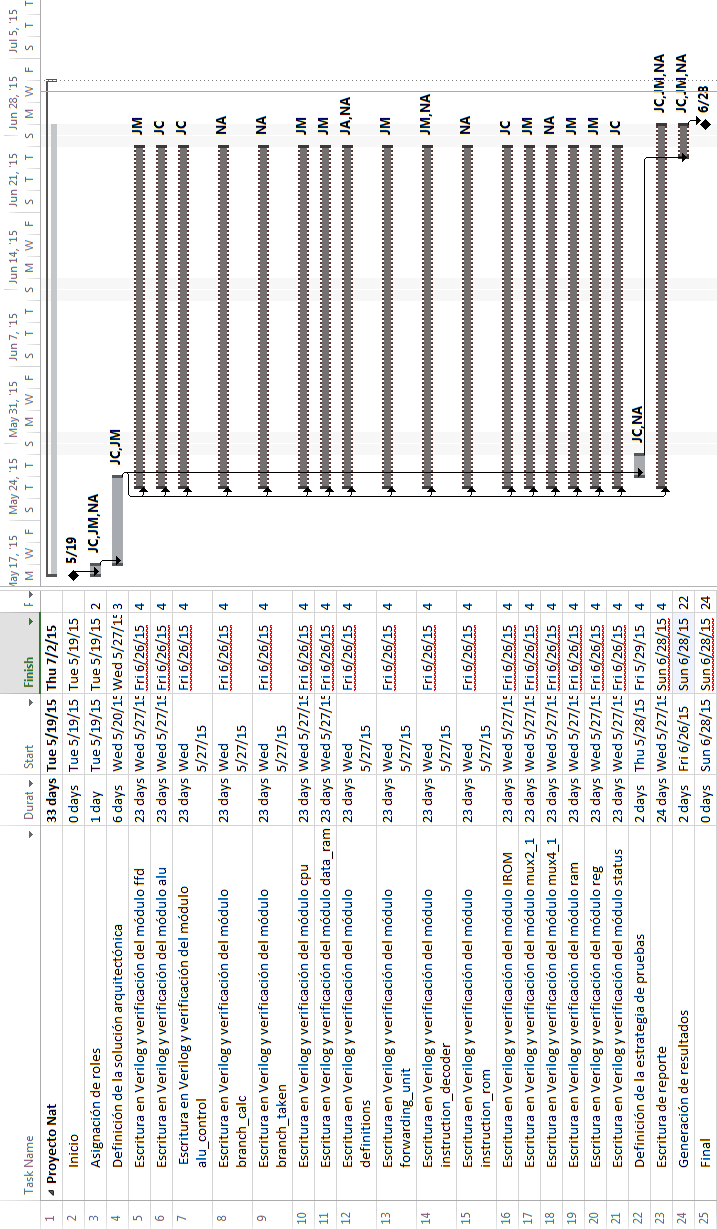
\includegraphics[scale=0.6]{imagenes/original.PNG}
\label{f:gannt_propuesto}
\end{figure}


\begin{figure}[hbtp]
\caption{Diagrama de Gannt Real}
\centering
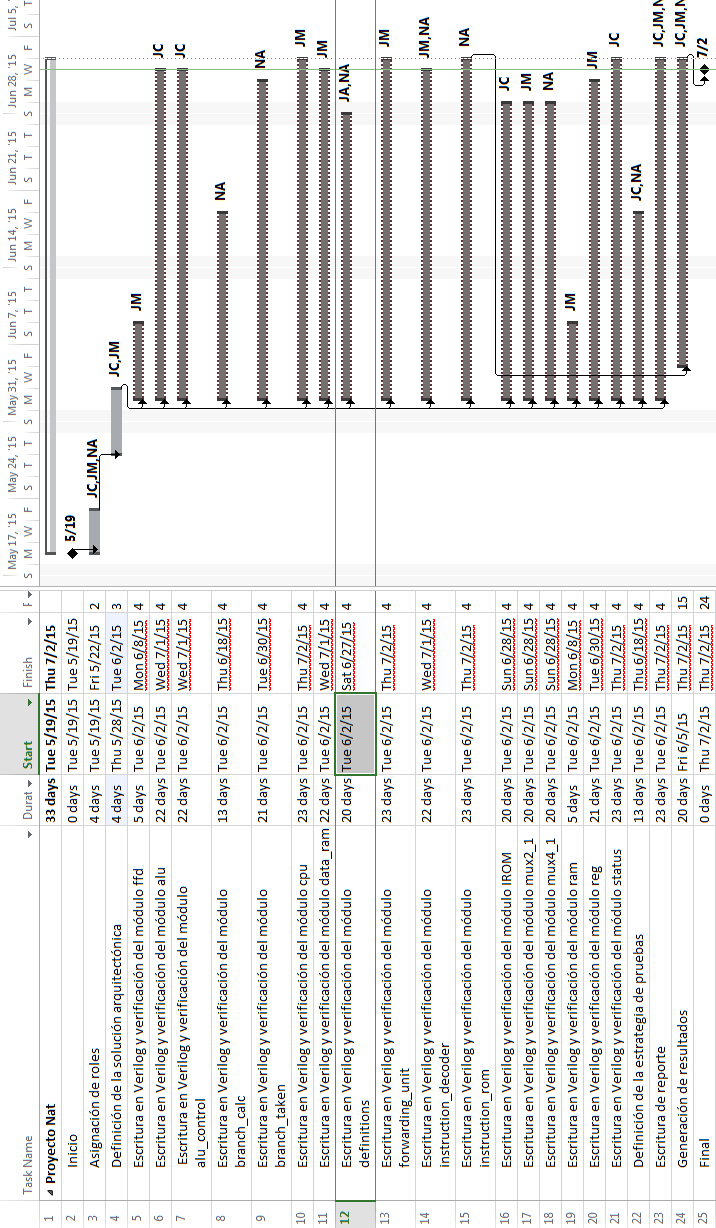
\includegraphics[scale=0.6]{imagenes/real.PNG}
\label{f:gannt_real}
\end{figure}

%%%%%%%%%%%%%%%%%%%%%%%%%%%%%
